\documentclass[11pt, aspectratio=169, table]{beamer}



\usepackage[utf8]{inputenc}
\usepackage{amsmath}
\renewcommand{\footnotesize}{\scriptsize}
\setbeamertemplate{footline}[frame number]
\usepackage{ulem}
\usepackage{programs}

\usepackage{multirow}
\usepackage{tabularx}

\usepackage{fretish}

\usepackage{appendixnumberbeamer}

\setbeamertemplate{background canvas}[bottom=white!10,top=white!10]

\usefonttheme[onlysmall]{structurebold}
%\useinnertheme{rounded}
\setbeamertemplate{itemize items}[triangle]


%%%tikzstuff
\usepackage{tikz}
\usetikzlibrary{shapes.geometric, arrows}
\tikzstyle{fragment} = [rectangle, minimum width=2em, minimum height=2em, text centered, draw=black, fill={rgb:black,1;white,3}]
\tikzstyle{req} = [rectangle, minimum width=2em, minimum height=2em, text centered, draw=black]
\tikzstyle{arrow} = [thick,->,>=stealth]


\usetheme{Madrid}
%\usetheme{Rochester}%
%\usetheme{JuanLesPins}%
%\usecolortheme{beaver}
%\usecolortheme{whale}%



\pdfpageattr {/Group << /S /Transparency /I true /CS /DeviceRGB>>}

%Corporate Brand of University 
\definecolor{UniBlue}{RGB}{0,55,113}
\definecolor{UniYellow}{RGB}{240,171,0}
\definecolor{UniRed}{RGB}{130,35,39}
\definecolor{UniGreen}{RGB}{0,103,120}

% set enumerations to squares, since balls look horrible in gold
\setbeamertemplate{enumerate item}[square]{}

% set color scheme to uni colours
\setbeamercolor{palette primary}{fg=UniYellow, bg=UniGreen}
\setbeamercolor{palette secondary}{fg=white, bg=UniBlue}
\setbeamercolor{palette tertiary}{fg=white, bg=UniRed}
\setbeamercolor{palette quaternary}{fg=white, bg=UniRed}

\setbeamercolor{structure}{fg=UniGreen}
% remove this if you want UniBlue items (or overwrite for something funky) 
\setbeamercolor{item}{fg=UniRed}

% the following lines overwrite the normal example and alert block colors
% even though these are "official" university brand colours, I am not a big
% fan of them... use them at your own discretion
% set color of alert
\setbeamercolor{block title alerted}{bg=UniRed!80!black}
% set color of example
\setbeamercolor{block title example}{bg=UniGreen!85!black}


\setbeamercolor{footbox1}{fg=UniYellow,bg=UniBlue}
\setbeamercolor{footbox2}{fg=UniYellow,bg=UniGreen}


%\setbeamertemplate{footline}[frame number]
\setbeamertemplate{footline}
{%
\begin{beamercolorbox}[wd=0.2\textwidth,ht=3ex,dp=1.5ex,leftskip=.5em,rightskip=.5em]{footbox1}%
\usebeamerfont{author in head/foot}%
\hspace{1em}\insertshortauthor%
\end{beamercolorbox}%
\vspace*{-4.5ex}\hspace*{0.2\textwidth}%
\begin{beamercolorbox}[wd=0.6\textwidth,ht=3ex,dp=1.5ex,center,leftskip=.5em]{footbox2}%
\usebeamerfont{title in head/foot}%
\centering
\insertshorttitle%
\end{beamercolorbox}%
\begin{beamercolorbox}[wd=0.2\textwidth,ht=3ex,dp=1.5ex,right,leftskip=.5em]{footbox1}%

\hfill\insertframenumber/\inserttotalframenumber\hspace{1em}
\end{beamercolorbox}

}

\setbeamertemplate{caption}[numbered]
\setbeamertemplate{itemize items}[triangle]



\setbeamertemplate{caption}[numbered]

\title[Sharper Specs for Smarter Drones]{Sharper Specs for Smarter Drones: \\Formalising Requirements with FRET} 

\date{10$^{th}$ of April 2025}

\author[]{\emph{Ois\'{i}n Sheridan} \and Leandro Buss Becker \and Marie Farrell \and Matt Luckcuck \and Rosemary Monahan}
\institute[]{
Department of Computer Science, Maynooth University/Hamilton Institute, Maynooth, Ireland
\and
Automation and Systems Department, Federal University of Santa Catarina, Florian\'{o}polis, Brazil
\and
Department of Computer Science, The University of Manchester, Manchester, UK
\and
School of Computer Science, University of Nottingham, Nottingham, UK
}


%% This adds a section heading slide is you use \section{}
\AtBeginSection[]{
  \begin{frame}
  \vfill
  \centering
  \begin{beamercolorbox}[sep=8pt,center,shadow=true,rounded=true]{title}
    \usebeamerfont{title}\insertsectionhead\par%
  \end{beamercolorbox}
  \vfill
  \end{frame}
}


%This removes the navigation symbols from the bottom of the slides
\setbeamertemplate{navigation symbols}{}


\begin{document}

%
\begin{frame}

\vspace{3mm}

\begin{minipage}{0.25\textwidth}
\begin{flushleft}

\includegraphics[height=4em]{images/mu-logo.png}
\end{flushleft}
\end{minipage}\noindent
\begin{minipage}{0.2\textwidth}
\centering

\includegraphics[height=4em]{images/UFSC-logo.png}
\end{minipage}\noindent
\begin{minipage}{0.27\textwidth}
\begin{flushright}

\includegraphics[height=4em]{images/manchester-logo.png}
\end{flushright}
\end{minipage}\noindent
\begin{minipage}{0.3\textwidth}
\begin{flushright}

\includegraphics[height=4em]{images/nottingham-logo.png}
\end{flushright}
\end{minipage}\noindent

\titlepage

\end{frame}



\begin{frame}{Introduction}

\begin{block}{Overview}

\begin{itemize}
    \item We describe the process of formalising the natural-language requirements for a tilt-rotor drone using the Formal Requirements Elicitation Tool (FRET).

    \item This requirements set evolved over four distinct versions as new information was elicited and incorporated into the FRETish specification.

    \item Our two concrete outputs are the formalised requirement set, which we will use in our ongoing development and verification of ProVANT; and metrics about the requirements.
    
    \item We present guidance for  requirements elicitation and formalisation with FRET.  
We highlight situations where it was difficult to formalise these requirements and describe potential improvements to FRET to address these difficulties.
	
\end{itemize}
\end{block}
\end{frame}

\section{Case Study -- ProVANT Emergentia Tilt-Rotor Drone}

\begin{frame}{Case Study -- Tilt-Rotor Drone}
\centering
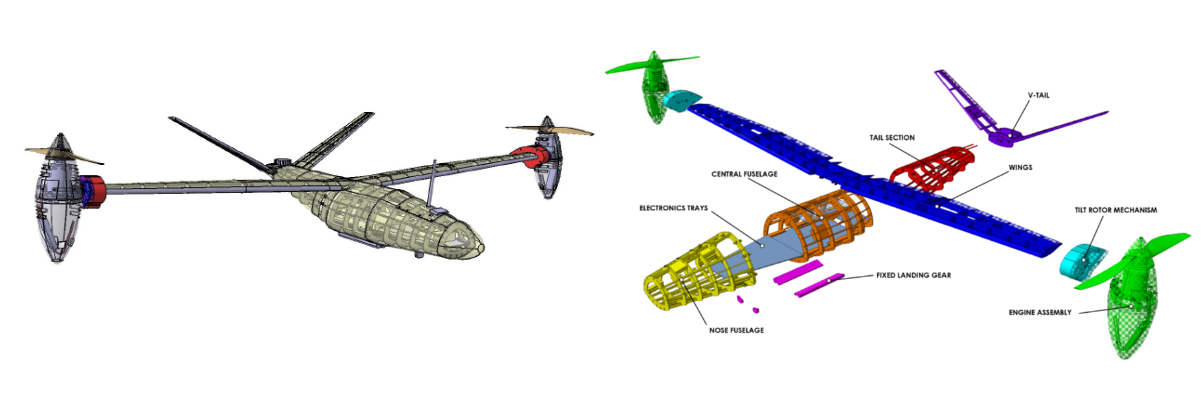
\includegraphics[width=\textwidth]{images/drone-overview.png}
\vspace{-8mm}
\begin{block}{}
	\begin{itemize}
		\item At the latter stage of development under the ProVANT Emergantia project
		
		\item The project is a collaboration among two Brazilian universities, Federal University of Minas Gerais (UFMG) and Federal University of Santa Catarina (UFSC), along with the University of Seville, Spain.
	\end{itemize}
\end{block}
\end{frame}

\begin{frame}{Case Study -- Tilt-Rotor Drone}
\begin{block}{}
	\begin{itemize}
		\item The drone can perform hovering and Vertical Take-off and Landing (VTOL) manoeuvres, as well as cruise flight as a fixed-wing aircraft.
		
		\item The architecture for the Drone's computing system comprises four main components:
		\begin{itemize}
		\item Raspberry Pi: Gathers sensor data and communicates with the Ground Control Station.
			\item Jetson: Processes sensor data and runs the control algorithm.
			\item Nucleos: the active nucleo interfaces with the drone's actuators and some sensors. Can also run a backup control algorithm in the case of a failure. There are two nucleos for reliability.
		\end{itemize}
		
		\item The set of requirements for the ProVANT Emergentia drone includes aspects related to:
		\begin{enumerate}
			\item operation features present during simulations and during real executions
			\item remote monitoring configurations
			\item timing constraints associated with the control loop
			\item operation modes under failure conditions
		\end{enumerate}
	\end{itemize}
\end{block}
\end{frame}

\section{Formalisation with FRET}

\begin{frame}{The Formal Requirements Elicitation Tool (FRET)}
\centering
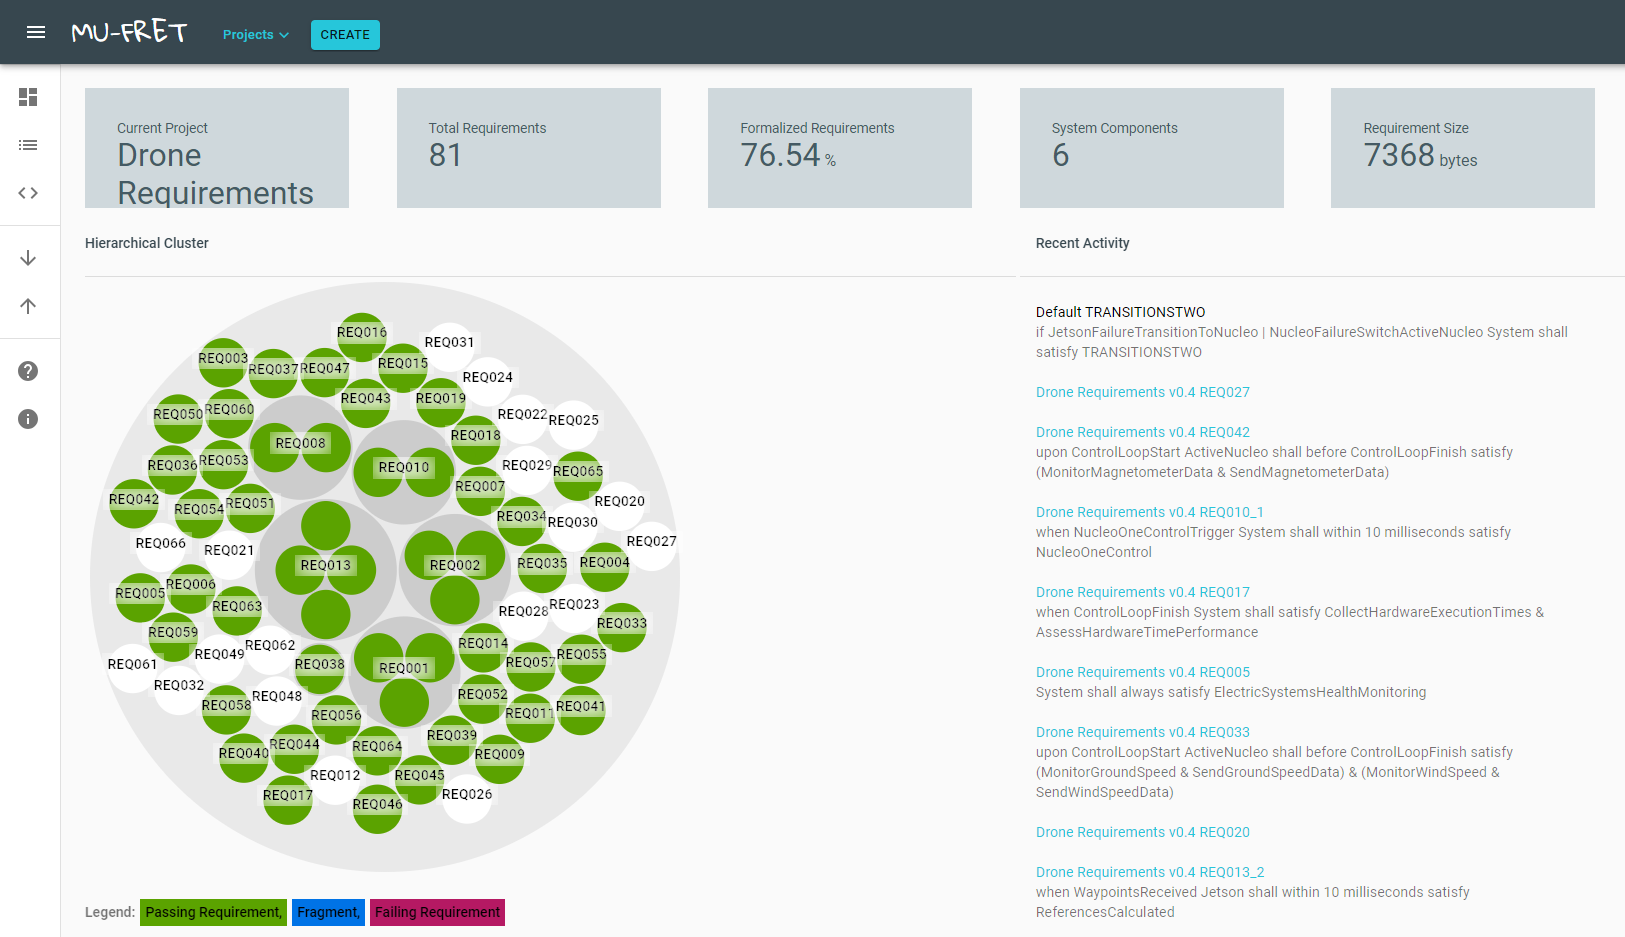
\includegraphics[width=0.8\textwidth]{images/mu-fret-dashboard.png}
\end{frame}


\begin{frame}{The Formal Requirements Elicitation Tool (FRET)}
\begin{minipage}{0.55\textwidth}
	\begin{block}{FRET}
		\begin{itemize}
			\item An open source tool for requirements engineering developed by NASA
			
			\item Requirements are written in a structured natural-language called FRETish
			
			\item FRET provides automated translations from FRETish to CoCoSpec contracts, which can be verified with the Kind2 model checker, and Copilot runtime monitors

                \item Formalised requirements are indicated in green, while those in white have not been formalised

		\end{itemize}
	\end{block}
\end{minipage}\noindent
\begin{minipage}{0.43\textwidth}
	\centering
	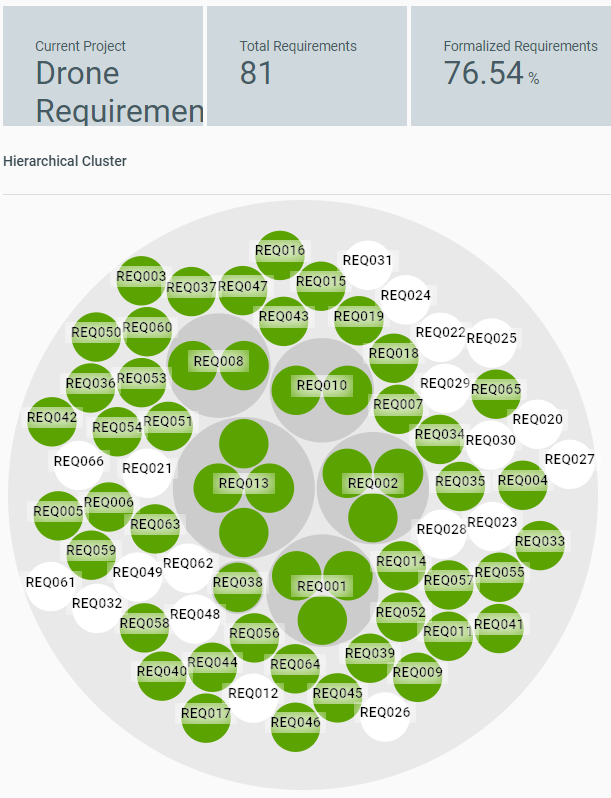
\includegraphics[width=0.86\textwidth]{images/drone-reqs-circle-diagram-no-legend.png}
\end{minipage}
\end{frame}


\begin{frame}
\centering
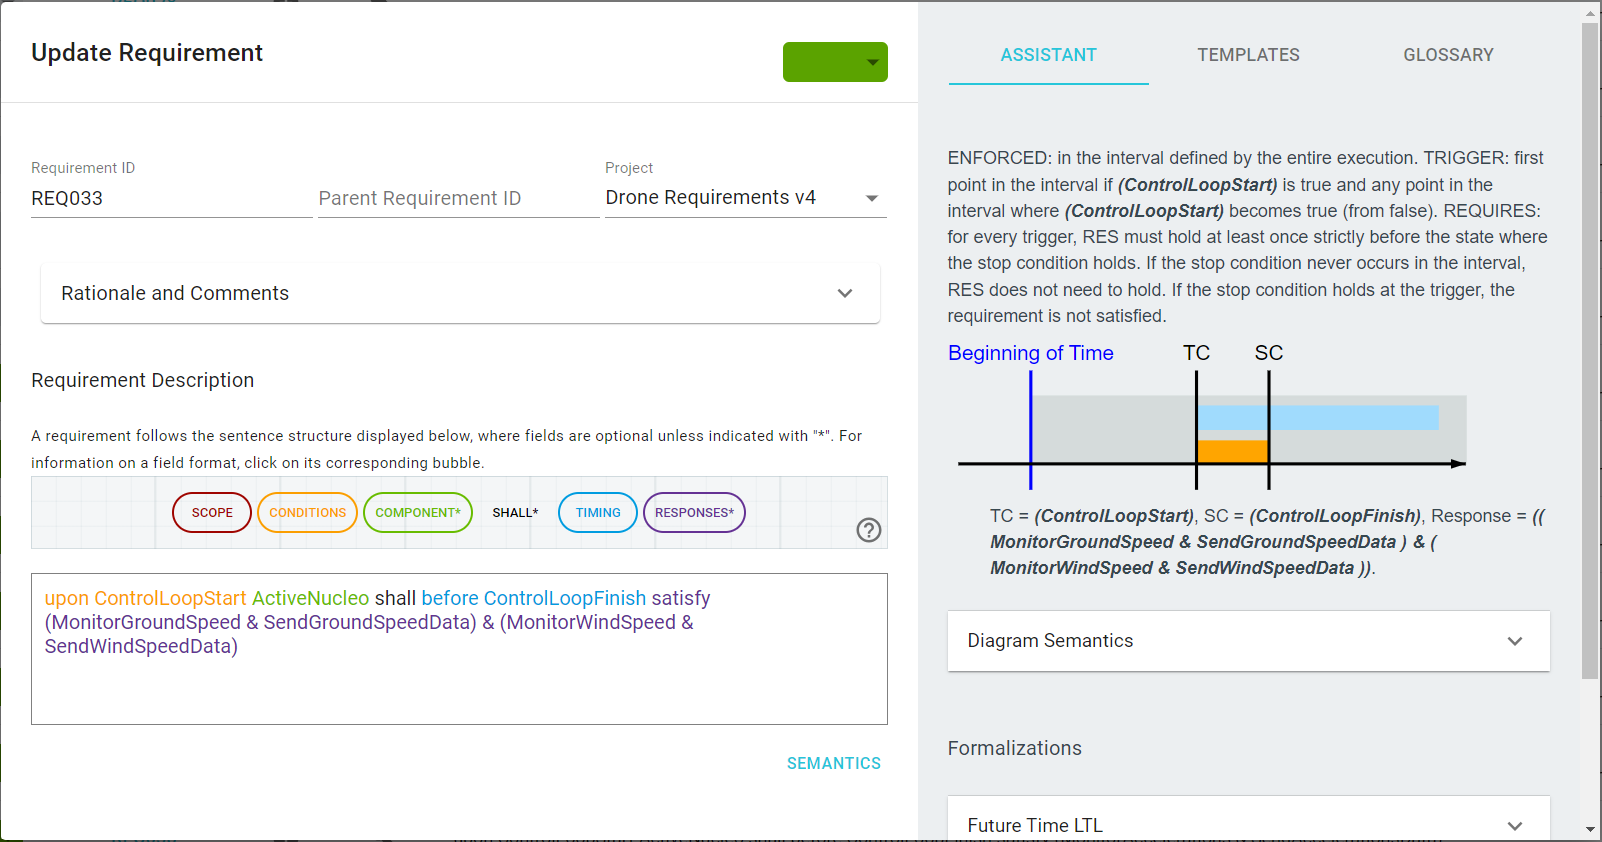
\includegraphics[width=\textwidth]{images/Drone-REQ033.png}
\end{frame}

\section{Formalising the Requirements}

\begin{frame}{Formalising the Requirements -- Methodology}
\centering
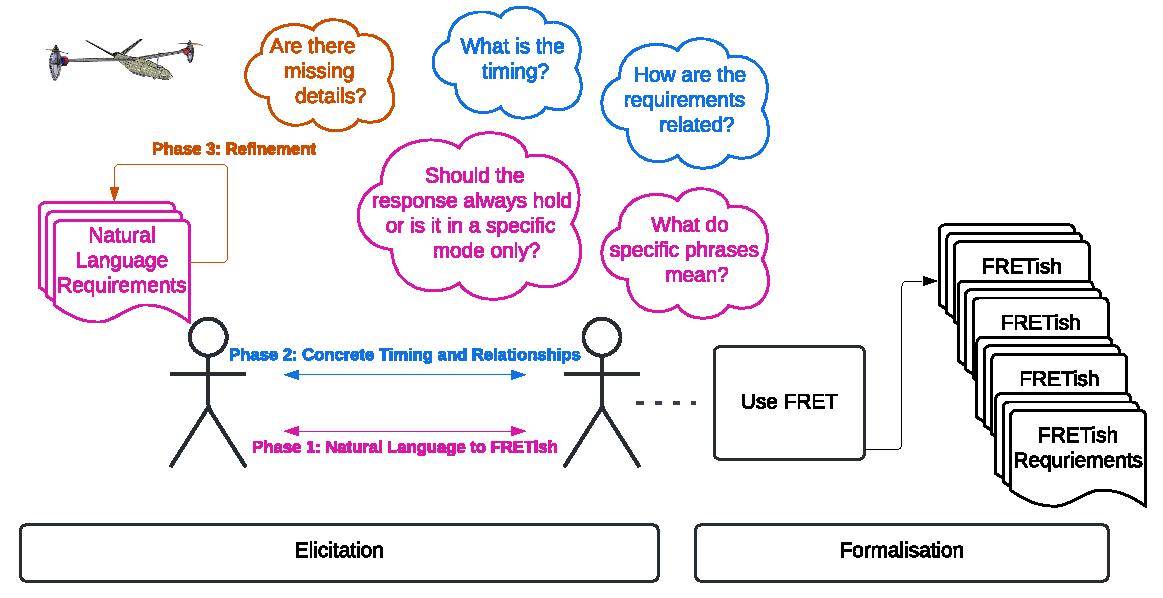
\includegraphics[width=0.9\textwidth]{images/processfinal.pdf}
\end{frame}


\begin{frame}{Formalising the Requirements -- Starting from Natural Language}
\begin{table}
    \centering
    \begin{tabular}{|p{0.11\textwidth}|p{0.82\textwidth}|}
    \hline
         \textbf{ID} & \textbf{Original English text} \\\hline
         \hline
         REQ001 & Allow failure simulations between nucleo/jetson and nucleo/nucleo \\\hline
         REQ013 & Send references \\\hline %Example of a requirement left out of V1 but that was formalised later (in V3)
		 REQ016 & Run each simulation loop within 10ms \\\hline        
         REQ018 & Present the total time spent \\\hline
         REQ019 & Present the time spent in the control algorithm \\\hline
         REQ024 & Work on any operational system \\\hline %This is an example of a non-functional requirement for Version 1
         REQ033 & Monitor linear velocities (ground speed and relative wind speed) \\\hline
         
    \end{tabular}
\end{table}

\begin{block}{}
\begin{itemize}
	\item The formalisation began with a set of 66 natural-language requirements for the tilt-rotor drone.
	
	\item Each requirement consists of an ID number and a short description
	
	\item Each one also had additional metadata: a \textit{Category} of Functional or Non-Functional, a \textit{Feasibility} ranging from Feasible to Unknown to Unfeasible, and a \textit{Group}.
\end{itemize}
\end{block}

\end{frame}

\begin{frame}{Formalising the Requirements -- FRETish Version 1}
\begin{block}{}
\begin{itemize}
	\item For the first iteration, we mapped the drone's  original natural-language requirements one-to-one into \fretish, matching the vocabulary between both versions where possible.
	
	\item Many of these were of a simple form, such as ``\component{System} shall \timing{always/eventually} \response{[variableName]}''
	
	\item Twenty of the 66 requirements were not translated in this initial set
	
	\item This stage gave us a clearer picture of what information we would need for a more robust formalisation
\end{itemize}
\end{block}

\begin{table}
	\centering
	\begin{tabular}{|p{0.11\textwidth}|p{0.82\textwidth}|}
		\hline
		\textbf{ID} & \textbf{FRETish First Iteration} \\\hline
		\hline
		REQ001 & \component{System} shall \timing{always} \response{AllowNucleoJetsonSimulation \& AllowNucleoNucleoSimulation} \\\hline
		REQ016 & \condition{when SimulationLoopStart} \component{System} shall \timing{within 10 milliseconds} \response{SimulationLoopFinish} \\\hline
		REQ033 & \component{System} shall \timing{always} \response{MonitorGroundSpeed \& MonitorWindSpeed} \\\hline
	\end{tabular}
\end{table}

\end{frame}

\begin{frame}{Formalising the Requirements -- FRETish Version 2}

\begin{block}{}
\begin{itemize}
	\item We discussed the ambiguities that we found and consulted with the use case provider for additional detail, leading to a number of updates.
	
	\item The largest update was a distinction between running the system in simulation versus in the real world. We created a \scopeX{SimulationMode} scope variable in nine requirements.
	
	\item 27 requirements gained a scope of ``\scopeW{MonitoringEnabled}'', so that Data Monitoring would be optional when running the system.
	
	\item We added the first child requirements to the set: REQ008\_1 \& \_2, and REQ010\_1 \& \_2.
\end{itemize}
\end{block}

\begin{table}
	\centering
	\begin{tabular}{|p{0.11\textwidth}|p{0.82\textwidth}|}
		\hline
		\textbf{ID} & \textbf{FRETish Second Iteration} \\\hline
		\hline
		REQ001 & \scope{SimulationMode} \component{System} shall \timing{eventually} \response{NucleoJetsonFailure|NucleoNucleoFailure} \\\hline
		REQ033 & \scopeW{MonitoringEnabled} \component{System} shall \timing{always} \response{MonitorGroundSpeed \& MonitorWindSpeed} \\\hline
	\end{tabular}
\end{table}

\end{frame}


\begin{frame}{Formalising the Requirements -- FRETish Version 2}
\vspace{-1mm}
\begin{block}{Child requirements}
We use child requirements to express how a requirement should apply to different components or in different situations.

REQ008\_1 specifies that the Raspberry Pi should transmit the data to the ground station, while REQ008\_2 states that the Jetson should save the data and send it to the active Nucleo for evaluation
\end{block}

\begin{table}
    \centering
    \begin{tabular}{|p{0.11\textwidth}|p{0.82\textwidth}|}
        \hline
         \textbf{ID} & \textbf{Final FRETish text} \\\hline
         \hline
         \multirow{2}{*}{REQ008} & Save any desired simulation data \\\cline{2-2}
         & \scopeX{after SimulationMode} \component{System} shall \timing{within 100 ticks} \response{SimulationDataSaved} \\\hline
         REQ008\_1 & \scopeX{after SimulationMode} \component{Raspberry} shall \timing{within 100 ticks} \response{GroundStationReceivedData} \\\hline
         REQ008\_2 & \scopeX{after SimulationMode} \component{Jetson} shall \timing{within 100 ticks} \response{SimulationDataRecorded \& NucleoReceivedData} \\\hline
    \end{tabular}
\end{table}

\end{frame}


\begin{frame}{Formalising the Requirements -- FRETish Version 3}
\vspace{-2mm}
\begin{block}{}
\begin{itemize}
	\item We found that the ``\scope{SimulationMode}'' scope didn't fully capture the intention of testing a specific response, so we added \condition{Conditions} for this.
	
	\item We introduced 9 new child requirements to specify additional behaviour of some requirements.
\end{itemize}
\end{block}

\begin{table}
	\centering
	\begin{tabular}{|p{0.11\textwidth}|p{0.82\textwidth}|}
		\hline
		\textbf{ID} & \textbf{FRETish Third Iteration} \\\hline
		\hline
		REQ001 & \scope{SimulationMode} \condition{whenever SimulateFailureTransitions} \component{System} shall \timing{eventually} \response{JetsonFailureTransitionToNucleo | NucleoFailureSwitchActiveNucleo} \\\hline
		REQ001\_1 & \condition{when JetsonControl \& JetsonFailureTransitionToNucleoFailure} \component{System} shall \timing{within 100 ticks} \response{!JetsonControl \& NucleoControl} \\\hline
		REQ001\_2 & \condition{when NucleoOneControl \& NucleoFailureSwitchActiveNucleo} \component{System} shall \timing{within 100 ticks} \response{!NucleoOneControl \& NucleoTwoControl} \\\hline
		%REQ001\_3 & \condition{when NucleoTwoControl \& NucleoFailureSwitchActiveNucleo} \component{System} shall \timing{within 100 ticks} \response{!NucleoTwoControl \& NucleoOneControl} \\\hline
	\end{tabular}
\end{table}

\end{frame}


\begin{frame}{Formalising the Requirements -- FRETish Version 3}
\begin{block}{}
\begin{itemize}
	\item The biggest change in this iteration: we decided to update two of the natural-language requirements - REQ018 and REQ019 - to capture new information.
	
	\item These were changed to include details about the timing of the control loop and control algorithm in the \fretish requirements, which was revealed in the elicitation discussions to be important information.
	
	\item Having this information captured in the \fretish was useful when developing the fourth iteration of the requirements.
\end{itemize}
\end{block}

\begin{table}
	\centering
	\begin{tabular}{|p{0.11\textwidth}|p{0.82\textwidth}|}
		\hline
		\textbf{Iteration} & \textbf{Natural-language and FRETish for REQ018} \\\hline
		\hline
		\multirow{2}{*}{Version 1} & Present the total time spent \\\cline{2-2}
		& \component{System} shall \timing{always} \response{DisplayTotalTimeSpent} \\\hline
		\multirow{2}{*}{Version 3} & The control loop will complete within 12 milliseconds \\\cline{2-2}
         & \condition{upon ControlLoopStart} \component{System} shall \timing{within 12 milliseconds} \response{ControlLoopFinish} \\\hline
		
	\end{tabular}
\end{table}

\end{frame}


\begin{frame}{Formalising the Requirements -- FRETish Version 4}

\begin{block}{}
\begin{itemize}
	\item This (currently) final iteration focused on cleaning up issues that arose during elicitation discussions and re-evaluation of the overall progress made up to that point.
	
	\item We returned to the Data Monitoring requirements and found that the idea of the system being run with or without monitoring was incorrect; the system should always monitor these values and transmit the data back to the GCS.
	
	\item We used the previous updates to REQ018 to update 23 monitoring requirements from a simple \timing{always} timing to a more detailed structure.
\end{itemize}
\end{block}

\begin{table}
	\centering
	\begin{tabular}{|p{0.11\textwidth}|p{0.82\textwidth}|}
		\hline
		%\textbf{} & \textbf{REQ060} \\\hline
		%\hline
		\textbf{REQ060} & Monitor current consumption in each voltage bus \\\hline
		\fretish v2 & \scopeW{MonitoringEnabled} \component{System} shall \timing{always} \response{MonitorVoltageBusConsumption} \\\hline
		\fretish v4 & \condition{upon ControlLoopStart} \component{ActiveNucleo} shall \timing{before ControlLoopFinish} \response{MonitorVoltageBusConsumption \& SendVoltageBusConsumptionData} \\\hline
		
	\end{tabular}
\end{table}

\end{frame}


\begin{frame}{Formalising the Requirements -- Beginning and End}
\vspace{-1mm}
\begin{table}
    \centering
    \begin{tabular}{|p{0.11\textwidth}|p{0.82\textwidth}|}
        \hline
         \textbf{ID} & \textbf{Final FRETish text} \\\hline
         \hline
         \multirow{2}{*}{REQ001} & Allow failure simulations between nucleo/jetson and nucleo/nucleo \\\cline{2-2}
         & \scope{SimulationMode} \condition{whenever SimulateFailureTransitions} \component{System} shall \timing{eventually} \response{JetsonFailureTransitionToNucleo | NucleoFailureSwitchActiveNucleo} \\\hline
         \multirow{2}{*}{REQ018} & The control loop will complete within 12 milliseconds \\\cline{2-2}
         & \condition{upon ControlLoopStart} \component{System} shall \timing{within 12 milliseconds} \response{ControlLoopFinish} \\\hline
         \multirow{2}{*}{REQ019} & The control algorithm will complete within 6 milliseconds \\\cline{2-2}
         & \condition{upon ControlAlgorithmStart} \component{System} shall \timing{within 6 milliseconds} \response{ControlAlgorithmFinish} \\\hline
         \multirow{2}{*}{REQ033} & Monitor linear velocities (ground speed and relative wind speed) \\\cline{2-2}
         & \condition{upon ControlLoopStart} \component{ActiveNucleo} shall \timing{before ControlLoopFinish} \response{(MonitorGroundSpeed \& SendGroundSpeedData) \& (MonitorWindSpeed \& SendWindSpeedData)} \\\hline
         %REQ060 & \condition{upon ControlLoopStart} \component{ActiveNucleo} shall \timing{before ControlLoopFinish} \response{MonitorVoltageBusConsumption \& SendVoltageBusConsumptionData} \\\hline
    \end{tabular}
\end{table}
\end{frame}


\section{Analysis \& Discussion}

\begin{frame}{Analysis \& Discussion}
\begin{table}[t]
\centering
        \begin{tabular}{|c|p{0.89\textwidth}|}
        \hline
        \emph{scope-option} & null = 47, in/during = 6, while = 5, after = 4 \\\hline
        \emph{condition-option} & null = 17, trigger(\condition{when/if}) = 39, continual(\condition{whenever}) = 6 \\\hline
        \emph{timing-option} &  null/eventually = 4, always = 15, next = 1, within = 18, before = 24  \\\hline
        parent-child &  28 child requirements were assigned a parent requirement   \\\hline
        \multicolumn{2}{|l|}{66 natural-language requirements, of which 47 are expressed in \fretish.}   \\
        \multicolumn{2}{|l|}{An additional 15 child requirements were created, for a total of 81 requirements in FRET.} \\\hline
        \end{tabular}
\end{table}

\begin{block}{Requirement Metrics}
\begin{itemize}
	\item The above table contains metrics on the structure of the final \fretish requirements.
	
	\item The \Scope field was not often used, as the natural-language requirements did not specify any system modes. \Scope was mostly used for the \scopeX{SimulationMode}.

	\item Conversely, almost every requirement in the final requirement set has a defined \Timing, with the few that don't being unchanged from earlier versions of the requirements set.
\end{itemize}
\end{block}

\end{frame}


\begin{frame}{Analysis \& Discussion}
\begin{block}{Recommendations for formalising requirements}
\begin{itemize}
	\item Requirements elicitation and formalisation is best performed as an incremental process, where all parties involved regularly re-examine the requirements in the context of newly-elicited details and newly-uncovered questions.
	
	\item We found it very useful to maintain a system where distinct ``versions'' of the requirements set were created and then analysed, rather than a more continuous development process.
	
	\item We encourage requirements engineers to maintain detailed records of prior versions of requirements and the updates made to them, to inform discussions on future development as well as for traceability.
\end{itemize}
\end{block}
\end{frame}


\begin{frame}{Analysis \& Discussion}
\begin{block}{Improvements to FRET and other tools}
\begin{itemize}
	\item At the time, tracking multiple iterations of a \fretish requirements set was difficult, as the tool did not directly support renaming or cloning projects. The development team have since added cloning functionality.
	
	\item Parameterised requirements - which would allow the user to apply a single requirement structure to a number of different variables - would have reduced duplication for the 23 Data Monitoring requirements.
	
	\item FRET currently supports adding comments and rationale to requirements, but there is no way to add comments to a project as a whole. This would be useful to precisely define the meanings of variables and reduce reliance on external notes.
\end{itemize}
\end{block}
\end{frame}



\end{document}
